\subsection{NEXT-White results}
\label{sec.new}

\begin{figure}
  \begin{center}
    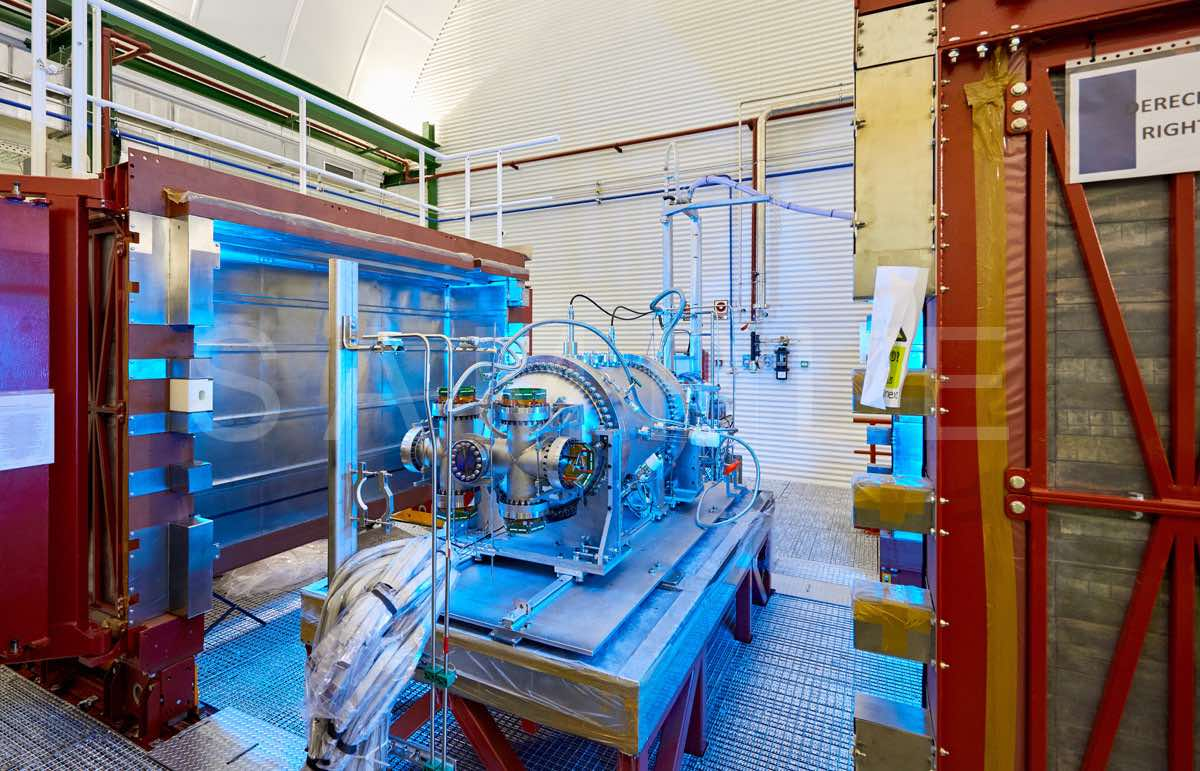
\includegraphics[width=0.55\textwidth]{img2/NEW.jpg}
    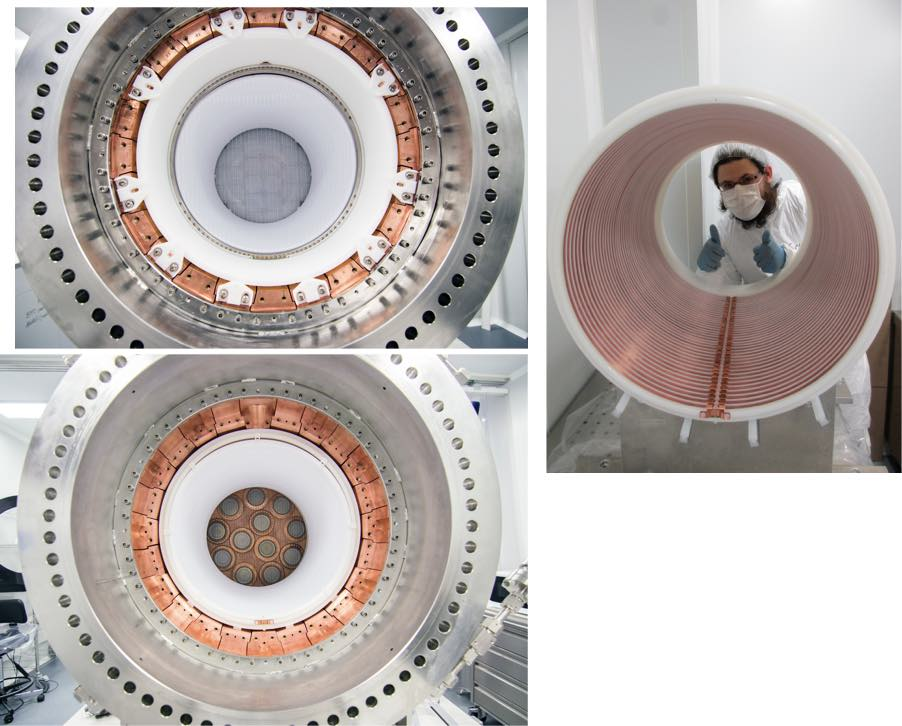
\includegraphics[width=0.40\textwidth]{img2/NEW2.jpg}
    \caption{The \NEW\ detector. Left: The apparatus, inside the lead shielding. Right: views of the inner detector, showing the energy plane, tracking plane and field cage.} 
    \label{fig:newd}
  \end{center}
\end{figure}

%--- data taking and quality ---%

The NEXT-White detector, shown in \fig\ \ref{fig:newd} is the first radiopure implementation of the NEXT technology. NEXT-White \cite{NEXT:2018rgj} was in stable operation at the LSC from October 2016 to July 2021, demonstrating unambiguously the excellent performance of the HPXe technology for \bbonu\ searches. Here, we present a brief summary of the main results achieved. 

%\indent

The first data taking periods (Run-I to Run-IV), using xenon gas depleted in \Xe{136} (2.6$\pm$0.2\%), were devoted to the detector commissioning and the measurement of the radiogenic backgrounds \cite{NEXT:2018zho,Novella:2019cne}. The data taking with gas enriched in \Xe{136} at 90.9$\pm$0.4\% (Run-V) started in February 2019 and ended in June 2020, with a total exposure of 271.6 days. The collected data have been used to achieve the main goals of this detector: an energy resolution of $\sim1\%$ FWHM at 2.6 MeV \cite{Renner:2019pfe}, an efficient discrimination between single and double-electron tracks by means of the event topology \cite{Ferrario:2019kwg,NEXT:2020jmz,NEXT:2021pjq}, and a measurement of the \Xe{136} \bbtnu~ half-life. In order to boost the significance of the \bbtnu ~observation, a new run with \Xe{136}-depleted gas (Run-VI) was taken between October 2020 and June 2021 (208.9 days), providing a direct measurement of the backgrounds with the same detector conditions as in Run-V. All data taking periods were divided into calibration (deployment of \Tl{208} and \Cs{137} sources) and low-background (no sources, lead shielding closed and radon abatement system in operation) phases. Along the different runs, the time stability of the NEXT-White detector was ensured by means of an extensive set of slow-controls and \Kr{83m} decays in the active volume. The krypton data were used to monitor the evolution of the electron lifetime ($\sim$13 ms at the end of Run-V and Run-VI), drift velocity ($\sim$0.92~mm/$\mu$s), light yield ($\sim$300 photo-electrons/keV), and energy resolution ($\sim$4\% FWHM at 41.5 keV).      

%--- energy resolution ---%
%\indent

The energy resolution of the NEXT-White detector has been measured at different energies, using \Cs{137} and \Th{228} calibration sources. The former provides 661.6 keV gamma rays, and the latter decays to \Tl{208} which provides gamma rays of 2614.5 keV. The \Kr{83m} decays, which occur uniformly in the whole volume of the detector, provide point-like energy depositions, which are used to map out the geometric variations in the sensor responses and electron lifetime of the detector. This map is used to correct the sensor response. A final correction is applied for an empirically observed dependence on the track orientation, which is very stable along the whole period of data taking. As shown in left panel of figure \ref{fig:newresults}, an energy resolution better than $1\%$ FWHM at 2614.5 MeV (above the $Q_{\beta\beta}$ of \Xe{136}, $\sim$2458 keV) has been measured in the fiducial volume, which comprises almost the entire volume of gas within the drift region \cite{Renner:2019pfe}.

%\indent


%--- topology-based event selection ---%
%The capability of distinguishing single from double electrons, characteristic of gaseous TPCs, is a powerful tool for background discrimination. In fact, the signal of a \bbonu decay consists of two electrons originating from the same vertex, while the background comes essentially from high energy gammas that convert in the detection material, producing Compton and photoelectric electrons. An electron releases its energy interacting with the gas molecules at an almost fixed rate, until the end of its range, where it produces a larger energy deposition in a smaller region.  Therefore, the signature of a \bbonu  event is a long track of constant energy deposition with two larger energy depositions at the end points (‘blobs’), while a background event shows only one blob at one extreme of the track. 
The reconstruction of the electron tracks in NEXT makes it possible to use the different topology of signal and background events to discriminate among them. In fact, the signature of a \bbonu ~event is a unique long track of constant energy deposition with two larger energy depositions at the end points (‘blobs’), while a background event shows typically more than one track, with only one blob at one extreme. 

%\indent


The NEXT-White detector has demonstrated the power of the topology-based event selection to discriminate background from signal, using the double-escape peak of \Tl{208}, originated by the interaction of the 2614.5 keV gamma rays when undergo pair production. The two 511 keV gammas emitted by the positron annihilation can escape the detector, or convert far enough as to be reconstructed as different tracks, and a peak at 1593 keV is visible in the energy spectrum, which represents the energy deposited by the electron-positron pair.  This energy deposition has the same topology as that of the two electrons of a \bbonu ~decay and can be studied to assess the power of topological discrimination, consisting in requiring the presence of two energy blobs at the extreme of the reconstructed track.  The first studies demonstrated a topological background rejection factor of $\sim$5, with 72\% signal efficiency \cite{Ferrario:2019kwg}. This was subsequently improved through the use of a deep convolutional neural network to yield a background rejection factor of  $\sim$10 with 65\% signal efficiency \cite{NEXT:2020jmz}. A second, significant improvement in topological performance compared to our first studies has been obtained using a more sophisticated reconstruction method, based on the Richardson-Lucy deconvolution algorithm. The algorithm allows reversing the blurring induced by electron diffusion and electroluminescence light production in the NEXT TPC. As shown in middle panel of \fig\ \ref{fig:newresults}, a  background rejection factor of 27 at 57\% signal efficiency has been measured in NEXT-White data \cite{NEXT:2021pjq}. Work is underway to combine both improvements, namely the Richardson-Lucy deconvolution algorithm with the use of deep convolutional neural networks, for potentially even larger gains.

%\indent


%--- measurement of the bb2nu decay rate ---%

A measurement of the \Xe{136} \bbtnu ~half-life has been achieved combining the \Xe{136}-enriched and \Xe{136}-depleted data samples, and relying on the topology-based $\beta\beta$-like selection. Two consistent results are derived from background-model-independent and background-model-dependent analysis approaches. In the first case, a novel technique in the field has been performed: a direct background subtraction by removing the Run-VI energy spectrum from the Run-V one. The background-subtracted observed rate yields a positive value that can be attributed to the \bbtnu ~events: R(\Xe{136})=250.8$\pm$82.6(stat)$\pm$28.5(sys) year$^{-1}$. Thus, a positive \bbtnu ~signal is observed at 2.9$\sigma$ from this rate-only measurement. In order to derive the half-life of the \Xe{136} \bbtnu\ from the background subtracted energy spectrum, a fit is performed to the corresponding MC expectation. The fit outcome is shown in right panel of \fig\ \ref{fig:newresults}, where the background-subtracted rate is superimposed to the best-fit \bbtnu ~MC. With a $\chi^{2}/dof$ of 16.1/21 (p-value=76\%), the fit yields a best-fit \bbtnu ~rate of R(\Xe{136})=291.0$\pm$72.7(stat)$\pm$27.5(sys) year$^{-1}$. This rate corresponds to a half-life of $\Ttnu=2.34^{+0.80}_{-0.46}(\textrm{stat})^{+0.30}_{-0.17}(\textrm{sys})\times10^{21}~\textrm{year}$. The rejection of the null hypothesis by means of the rate plus shape fit reaches 3.8$\sigma$ (4.1$\sigma$ expected). This result is cross-checked by a background-model-dependent analysis, in which the Run-V and Run-VI energy spectra are jointly fitted to their signal plus background expectations. In this approach, the \Tl{208}, \Bi{214}, \Co{60} and \K{40} decay rates are fitted along with the \bbtnu ~rate. The fit yields a best-fit value of R(\Xe{136})=334$\pm$78(stat)$\pm$54(sys) year$^{-1}$, corresponding to a half-life of $\Ttnu=2.14^{+0.65}_{-0.38}(\textrm{stat})^{+0.46}_{-0.26}(\textrm{sys})\times10^{21}~\textrm{year}$, with $\chi^2/dof$=146.1/114. Our results, already published as
a preprint \cite{nextcollaboration2021measurement}, have been submitted to Phys.~Rev.~Lett. 


\begin{figure}
  \begin{center}
    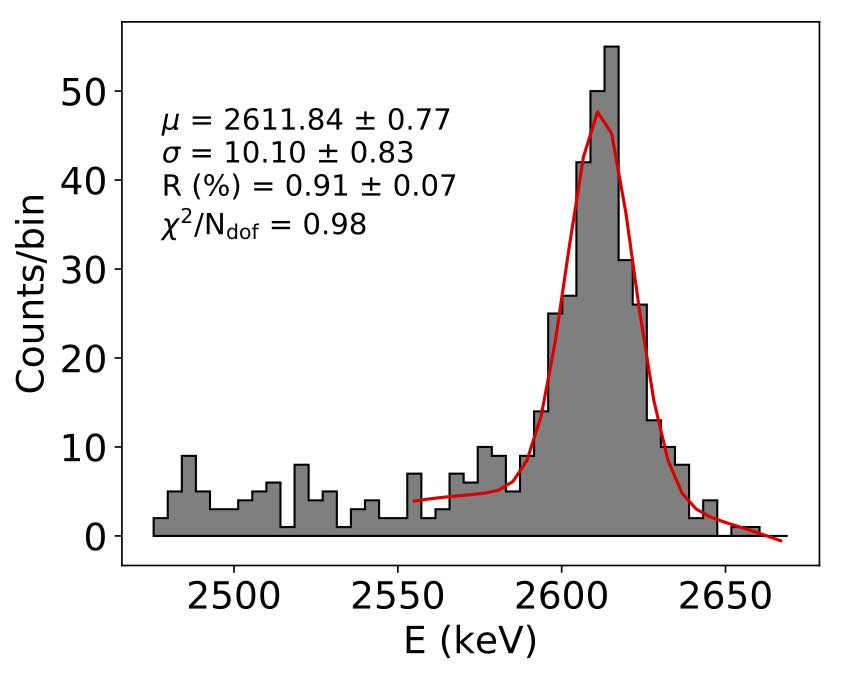
\includegraphics[width=0.31\textwidth]{img2/eres_tl208.jpg}
    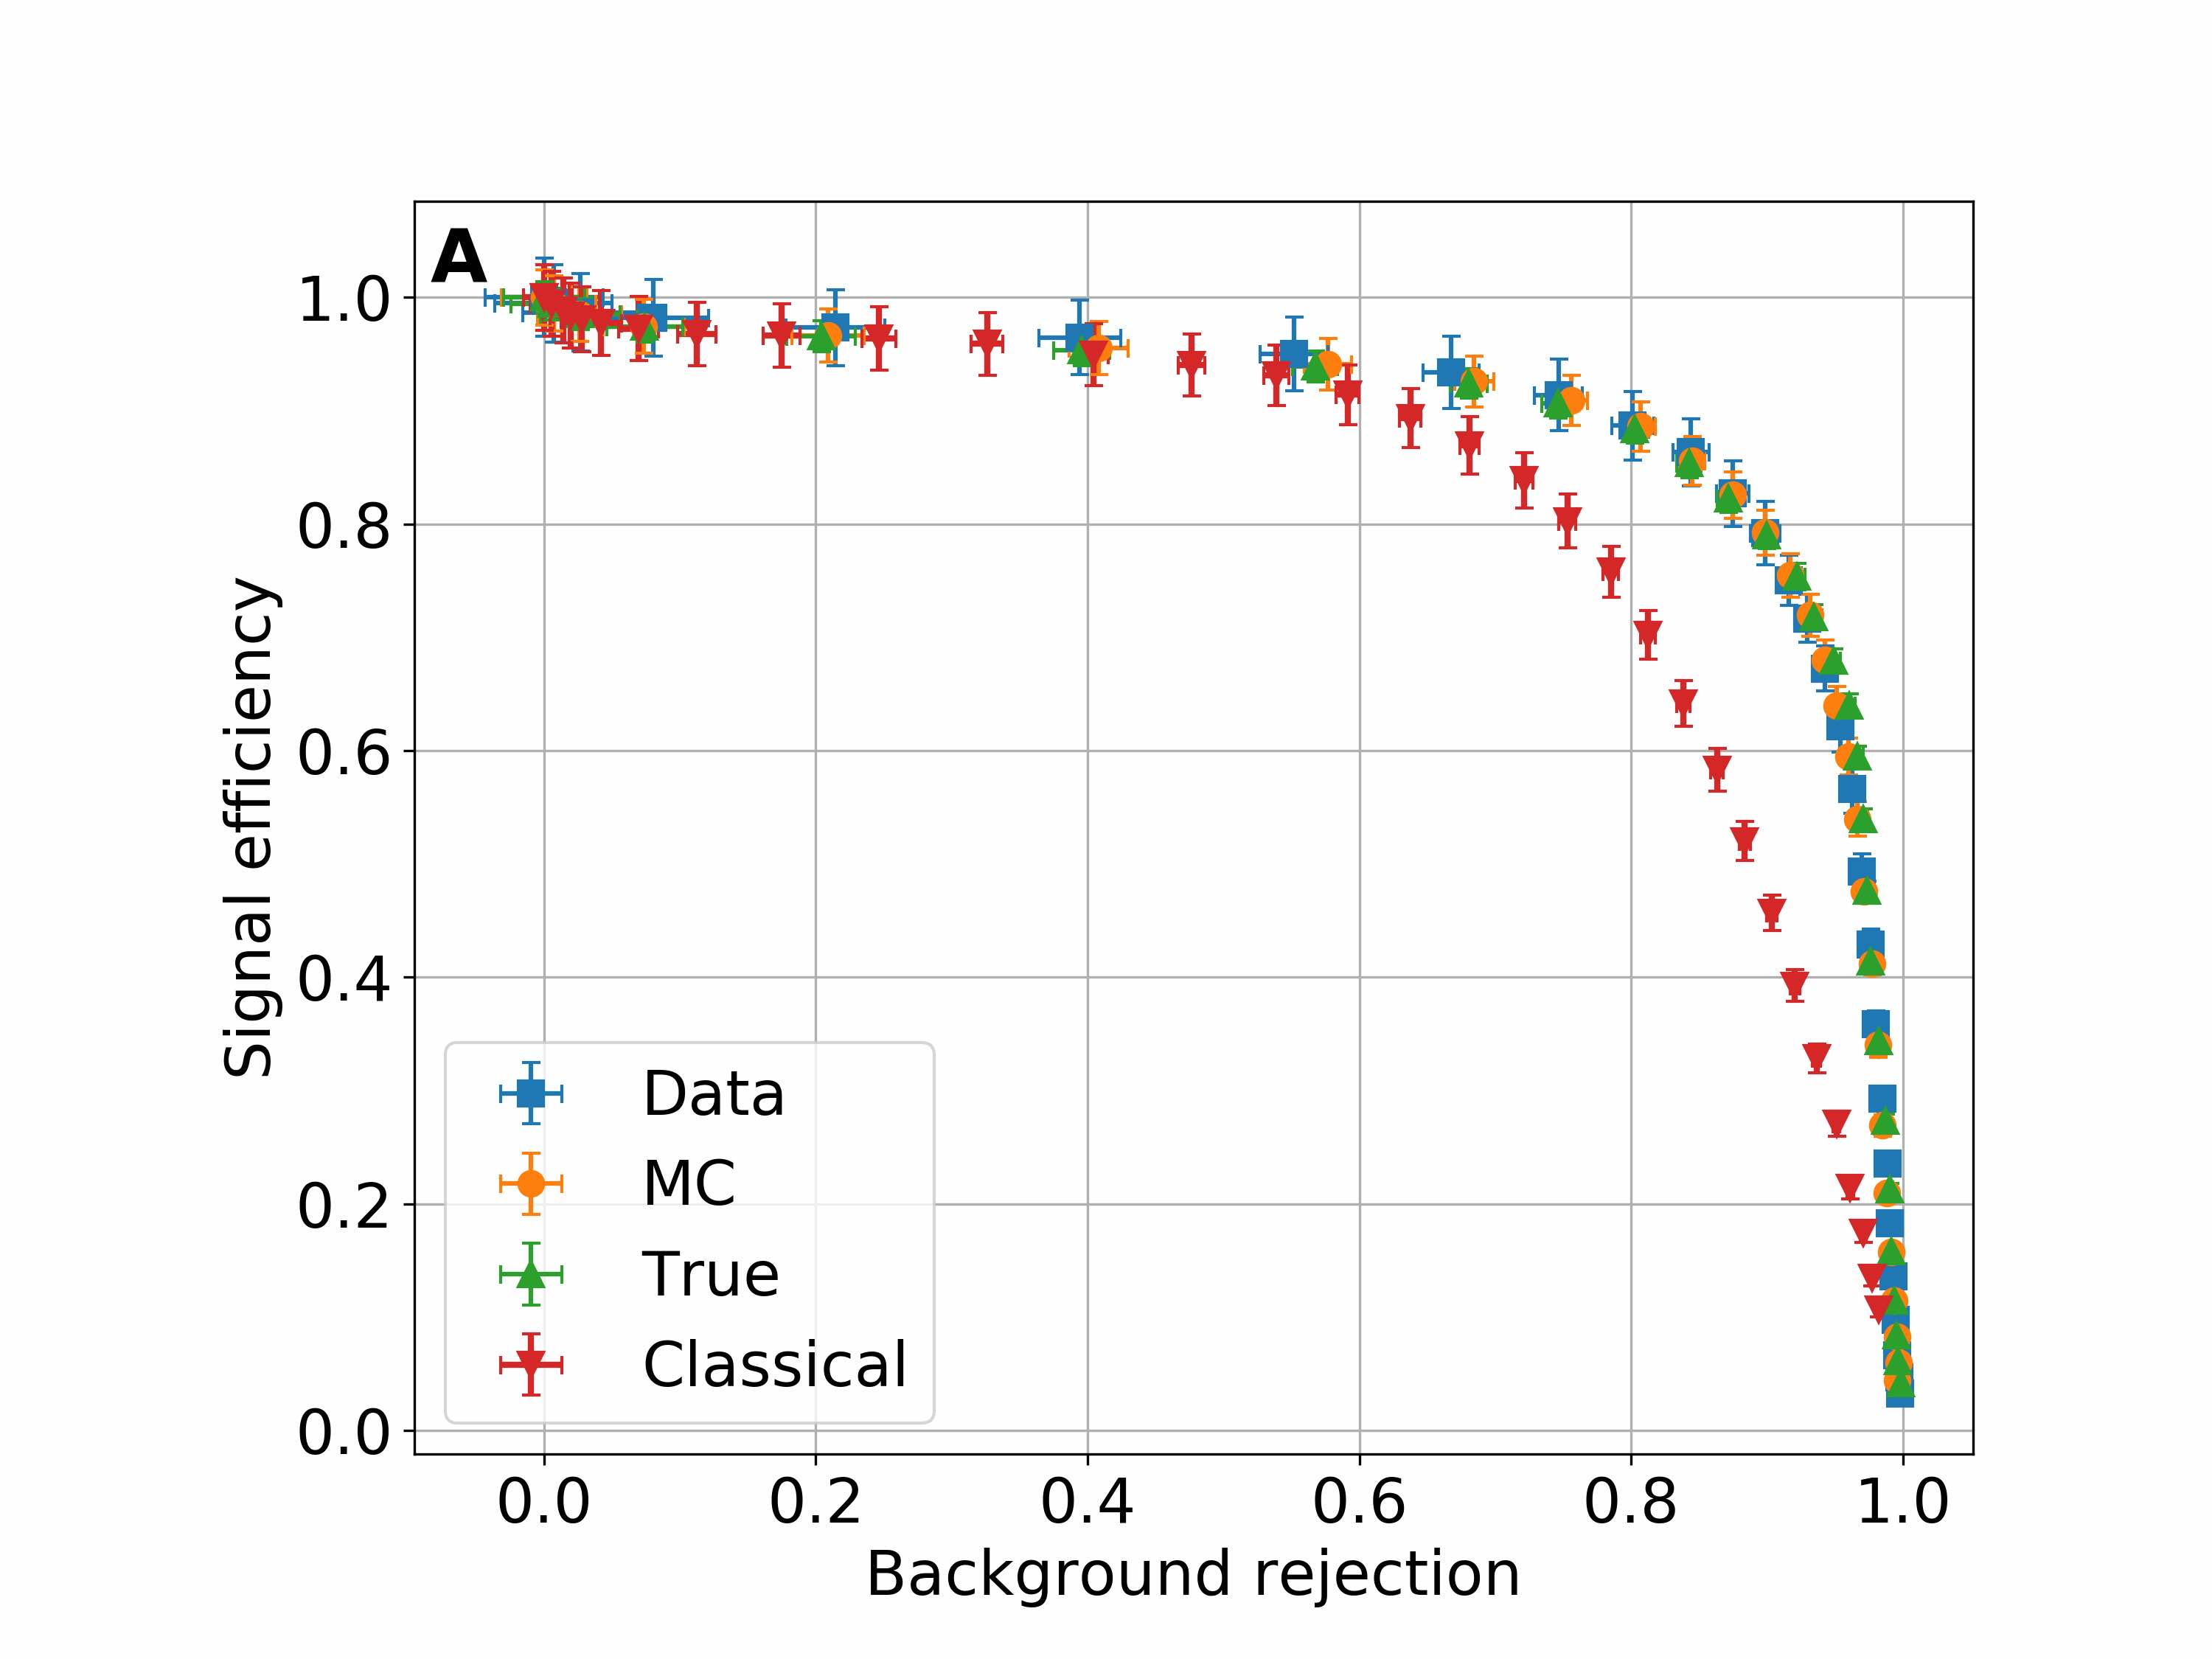
\includegraphics[width=0.36\textwidth]{img2/SigEffBGRej.jpg}
    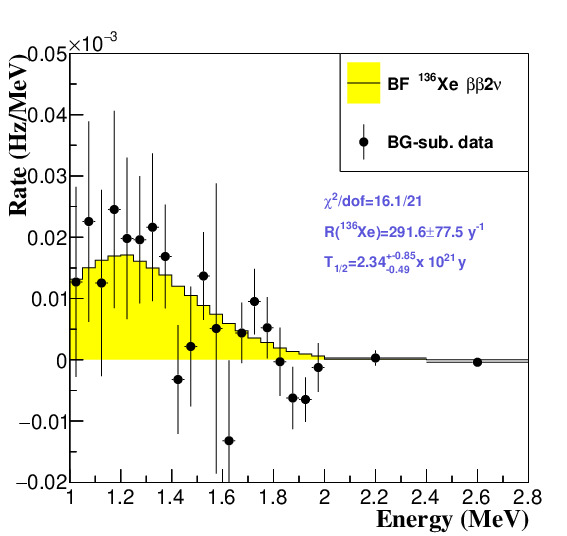
\includegraphics[width=0.31\textwidth]{img2/BGSubFit.jpg}
    \caption{Main NEXT-White results. Left: energy resolution at the 2.6 MeV \Tl{208} photo-peak (from \cite{Renner:2019pfe}). Middle: signal efficiency versus background rejection (from \cite{NEXT:2021pjq}). Right: Background-subtracted \bbtnu ~fit (from  \cite{nextcollaboration2021measurement}).} 
    \label{fig:newresults}
  \end{center}
\end{figure}


